
% * Week 1. (Jul 27) Introduction and R boot camp (Rob & Souhaib)
%   - Lecture 1:  What is Business Analytics? Show case of R.
%   - Lab 1: R exercises
%   - Lecture 2: Introduction to R programming
% - R, Rstudio
% - Rmarkdown
% - Examples:
%     prediction: bulldozers
%     classification: see JWHAT
%     clustering
%   Business analytics vs data science vs statistics vs econometrics 
%   Venn diagrams



\documentclass[14pt]{beamer}
\usepackage{pgf,tikz,pgfpages,amsmath,bm,fancyvrb,animate}
\usepackage{graphicx,bera,booktabs,multicol}
\usepackage[australian]{babel}
\usepackage[utf8]{inputenc}
\usepackage{media9}

\usepackage{verbatim}

\usepackage{wasysym}

\definecolor{Orange}{RGB}{255,140,0}
\long\def\TCorange#1{\textcolor{Orange}{#1}}
\long\def\TCblue#1{\textcolor{blue}{#1}}

\newcommand\Wider[2][3em]{%
\makebox[\linewidth][c]{%
  \begin{minipage}{\dimexpr\textwidth+#1\relax}
  \raggedright#2
  \end{minipage}%
  }%
}

\usetheme{Monash}
\def\ben{\begin{enumerate}[<+-| alert@+>]}
\def\een{\end{enumerate}}

%\AtBeginSubsection[]  
%  {  
%    \begin{frame}<*>{Outline}  
%      \tableofcontents[currentsection,currentsubsection]  
%    \end{frame}  
%  }


%\graphicspath{{../figures/}}
\graphicspath{{../figures/}{../figures/book_figures/Chapter2/}}


\title[Statistical learning]{Business Analytics}
\author{Week 2.\\ Statistical learning}
\date{3 August 2015}

\DefineShortVerb{\"}
\def\FancyVerbFormatCom{\color[rgb]{0.6,0,1}\relax}


\def\source#1{\vspace{-0.4cm}\par{\fontsize{6}{8}\sffamily \url{#1}}}
\def\inlinesource#1{\hbox{\fontsize{6}{8}\sffamily \url{#1}}}

%\newcommand{\lol}{\smiley}
%\newcommand{\nlol}{\frownie}
\definecolor{darkgreen}{rgb}{0,0.39,0}


 
\begin{document}

\begin{frame}[plain]{}
\maketitle
\begin{textblock}{11}(0.5,1.3){\color{white}\large
\textbf{ETC3250}}
\end{textblock}


\end{frame}

\begin{frame}{Learning from data}

\begin{itemize}

\item \textbf{Better understand} or \textbf{make predictions} about a certain
phenomenon under study

\item \textbf{Construct a model} of that phenomenon by finding relations between several variables

\item If phenomenon is complex or depends on a large number of variables, an \textbf{analytical solution} might not be available

\item However, we can  \textbf{collect data} and learn a model that  \textbf{approximates} the true underlying phenomenon

\end{itemize}

\end{frame}

\begin{frame}{Learning from a dataset}

\centerline{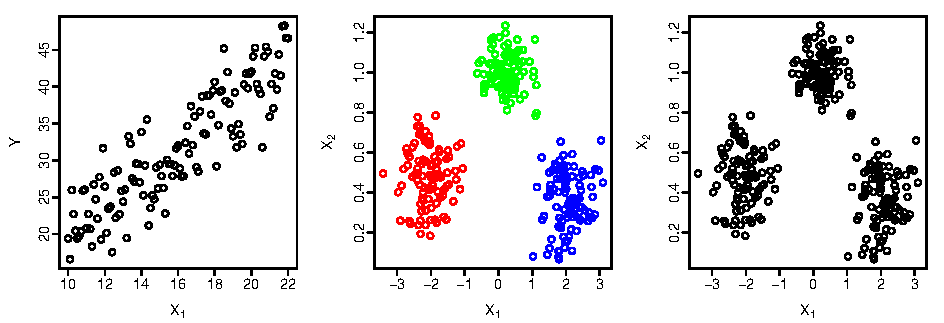
\includegraphics[width=12.2cm]{statlearn.pdf}}

$$ \mathcal{D} = \{(x_i, y_i)\}_{i = 1}^N \text{~with~} x_i = (x_{i1}, \dots, x_{ip})^{T}$$

\pause
\begin{block}\small
\textbf{Statistical learning} provides a framework for constructing models from $\mathcal{D}$.
\end{block}

\end{frame}

\begin{frame}{Different learning problems}

\begin{itemize}
	\item Supervised learning 
		\begin{itemize}
		\item Regression (or prediction)
		\item Classification
		\end{itemize}
	$\rightarrow$ $y_i$ \textcolor{red}{available for all} $x_i$
	\item Unsupervised learning \\
	$\rightarrow$ $y_i$ \textcolor{red}{unavailable for all} $x_i$
	\item Semi-supervised learning \\
	$\rightarrow$ $y_i$ \textcolor{red}{available only for few} $x_i$
	\item Other types of learning: reinforcement learning, online learning, active learning, etc. 
\end{itemize}

Identification of the best learning problem is important in practice

\end{frame}

\begin{frame}{What is Statistical Learning?}\large

$ \mathcal{D} = \{(x_i, y_i)\}_{i = 1}^N$

$$Y=f(\overbrace{X_1, \dots, X_p}^{X}) + \varepsilon$$

\begin{itemize}
	\item $Y$: response (output)
	\item $f$: unknown function
	\item $X$: set of $p$ predictors (inputs)
	\item $\varepsilon$: error term
\end{itemize}

\centerline{\textcolor{red}{Learn (or estimate) the function $f$ using $\mathcal{D}$}}

\vspace{.5cm}

\end{frame}

\begin{frame}{What is Statistical Learning?}\large


\placefig{0.2}{1}{width=12.2cm}{2-2.pdf}

\end{frame}

\begin{frame}{What is Statistical Learning?}\large


\placefig{1.3}{1}{width=10cm}{2-3.pdf}

\end{frame}


\begin{frame}{Why estimate $f$?}
\vspace{-0.5cm}
%\centerline{ 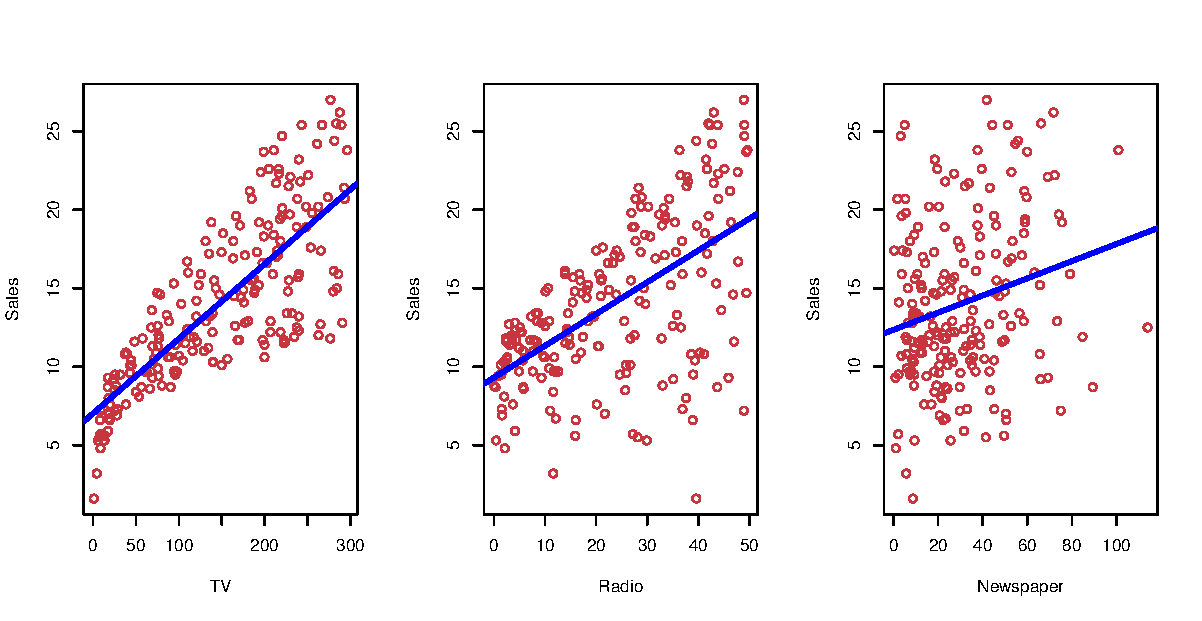
\includegraphics[width = .9\textwidth]{2-1.pdf}}

\begin{itemize}
	\item Prediction: $ \hat Y = \hat f(X)$

\begin{align*}
	\text{E}[(Y - \hat Y)^2] &= \text{E}[(f(X) + \varepsilon - \hat Y)^2] \\
					  &= \underbrace{\text{E}[(f(X) - \hat f(X))^2]}_{\text{Reducible}} + \underbrace{\text{Var}(\varepsilon)}_{\text{Irreducible}}
\end{align*} 
	
	\item Inference (or explanation):
	\begin{itemize}
	\item Which predictors are associated with the response?
	\item What is the relationship between the response and each predictor?
	\end{itemize}
\end{itemize}

\end{frame}

\begin{frame}{How do we estimate $f$?}

\begin{itemize}
	\item \textbf{Parametric methods}
		\begin{itemize}
		\item Assumption about the form of $f$, e.g. linear: $\textcolor{blue}{f(X) = \beta_0 + \beta_1 X_1 + \dots + \beta_p X_p} \text{~and~} \textcolor{blue}{\hat Y(x) = \hat f(x)} $
		\item[\textcolor{darkgreen}{\smiley}] The problem of estimating $f$ reduces to estimating a set of parameters
		\item[\textcolor{darkgreen}{\smiley}] Usually a good starting point for many learning problems
		\item [\textcolor{red}{\frownie}] Poor performance if linearity assumption is wrong
		\end{itemize}
	\item \textbf{Non-parametric methods}
		\begin{itemize}
		\item No \emph{explicit} assumptions about the  form of $f$, e.g. nearest neighbours: $\textcolor{blue}{\hat Y(x) = \frac1k \sum_{x_i \in N_k(x)} y_i}$
		\item[\textcolor{darkgreen}{\smiley}] High flexibility: it can potentially fit a wider range of shapes for $f$
		\item [\textcolor{red}{\frownie}] A large number of observations is required to estimate $f$ with good accuracy
		\end{itemize}
\end{itemize}

\end{frame}


\begin{frame}{How do we estimate $f$?}
\vspace{.5cm}

  \begin{columns}
    \begin{column}{0.5\textwidth}
      \centering
      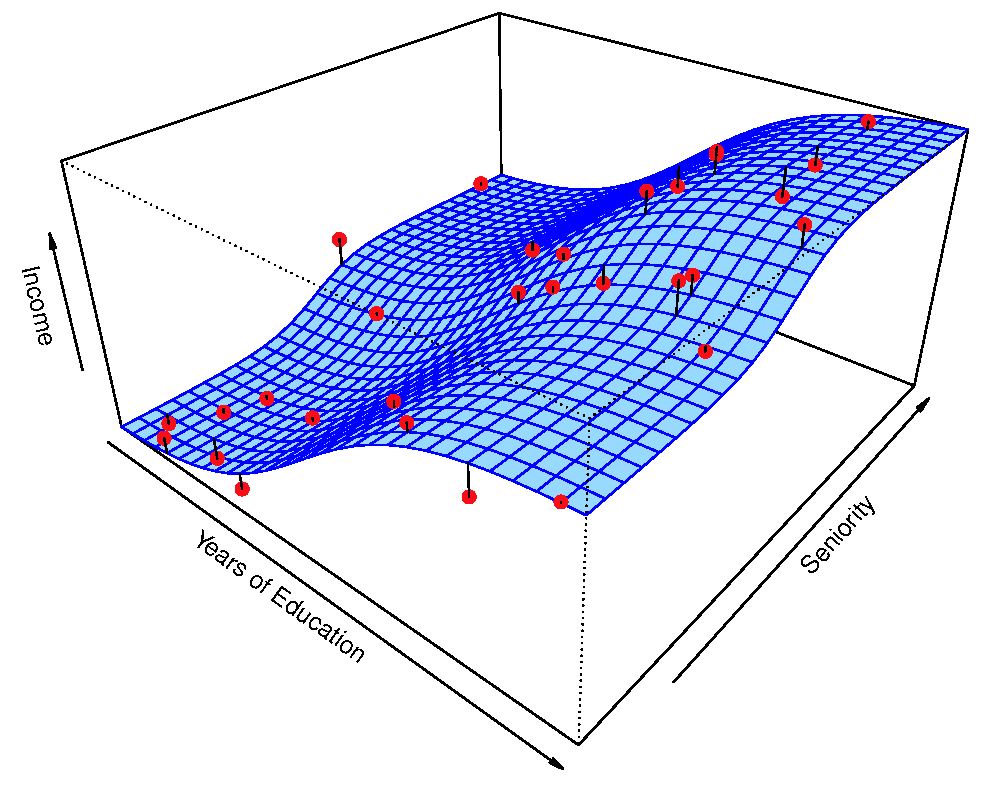
\includegraphics[width = \textwidth]{2-3.pdf}
    \end{column}
    \begin{column}{0.5\textwidth}
      \centering
      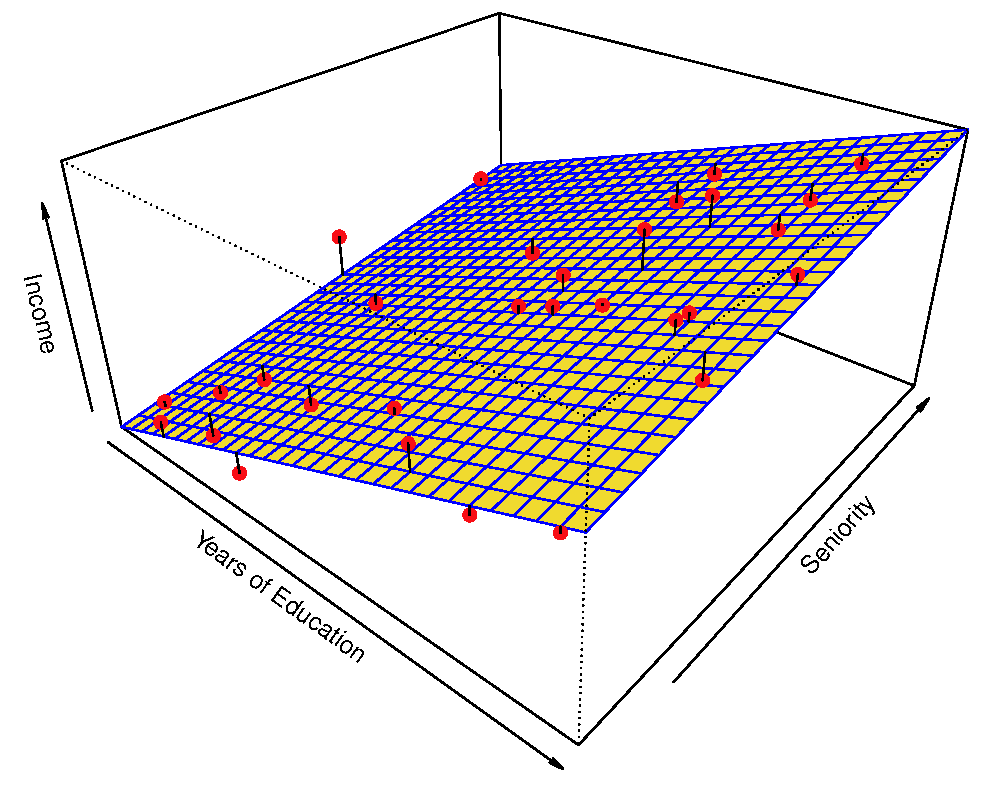
\includegraphics[width = \textwidth]{2-4.pdf}
    \end{column}
  \end{columns}
  
  \vspace{.5cm}
  {\small $ \hat f(\text{\textcolor{orange}{education}}, \text{\textcolor{orange}{seniority}}) = \hat \beta_0 + \hat \beta_1 \times \text{\textcolor{orange}{education}} + \hat \beta_2 \times \text{\textcolor{orange}{seniority}} $}
\end{frame}

\begin{frame}{How do we estimate $f$?}
\vspace{.5cm}

  \begin{columns}
    \begin{column}{0.5\textwidth}
      \centering
      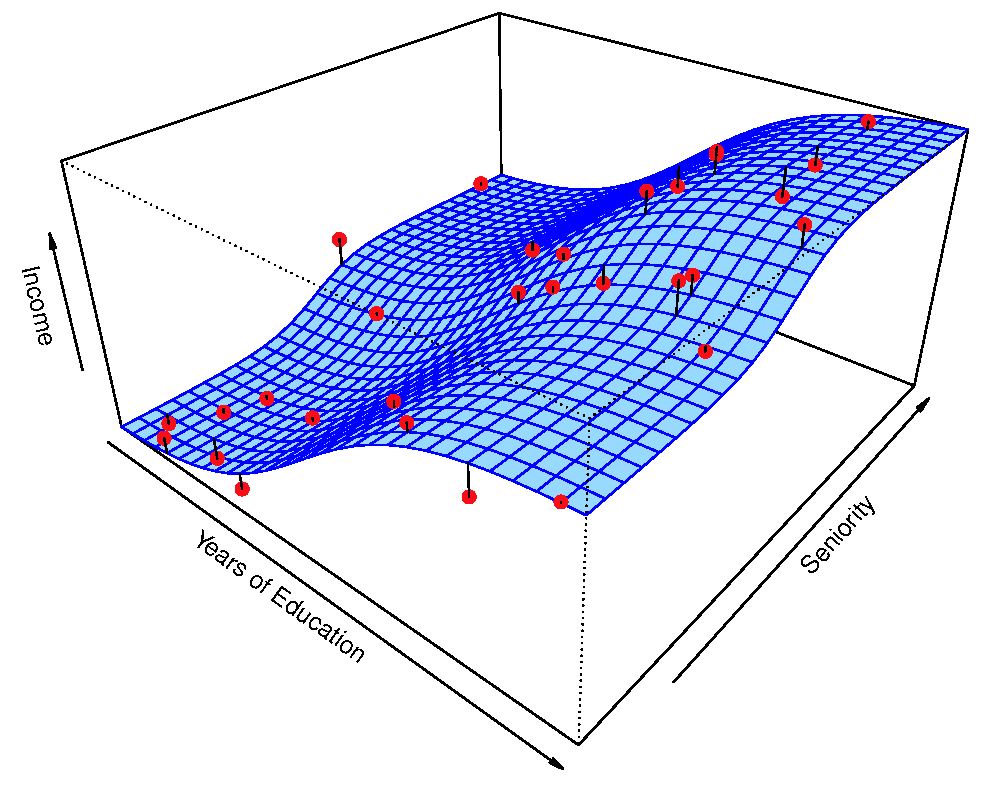
\includegraphics[width = \textwidth]{2-3.pdf}
    \end{column}
    \begin{column}{0.5\textwidth}
      \centering
      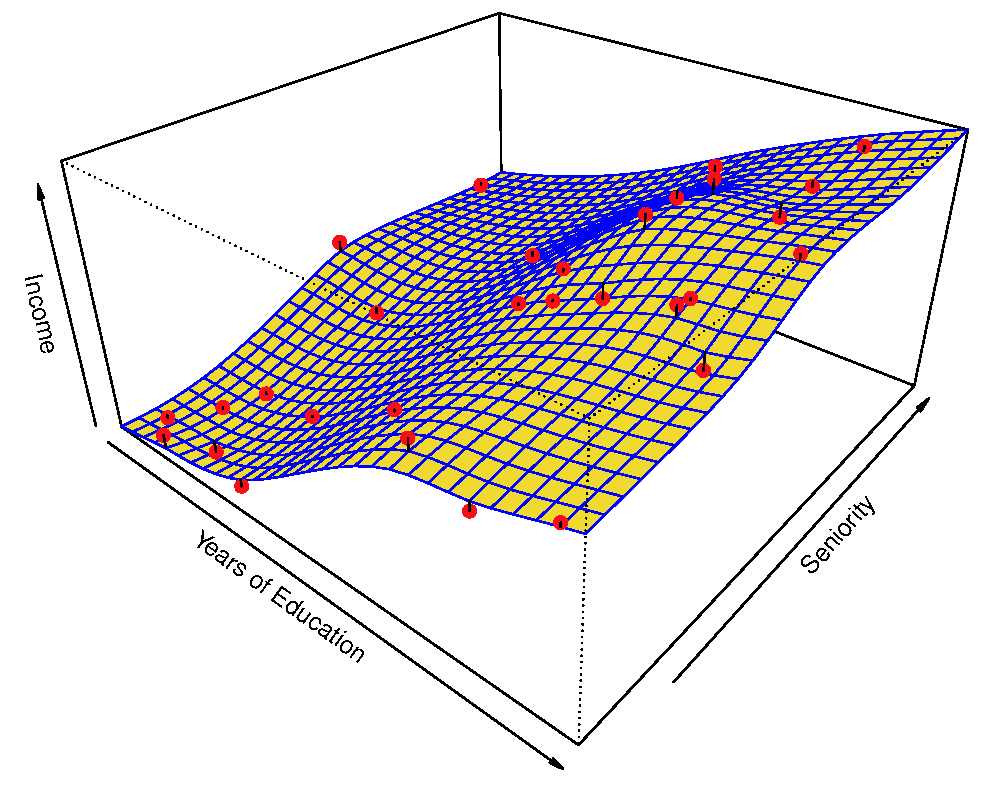
\includegraphics[width = \textwidth]{2-5.pdf}
    \end{column}
  \end{columns}
\end{frame}

\begin{frame}{How do we estimate $f$?}
\vspace{.5cm}

  \begin{columns}
    \begin{column}{0.5\textwidth}
      \centering
      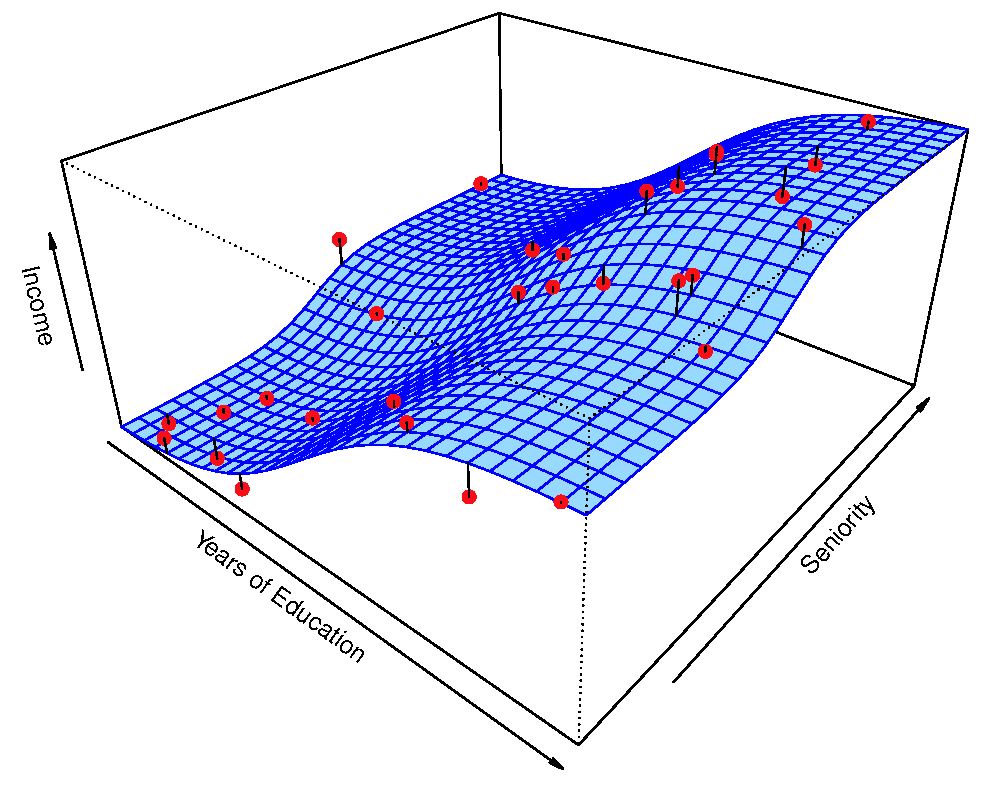
\includegraphics[width = \textwidth]{2-3.pdf}
    \end{column}
    \begin{column}{0.5\textwidth}
      \centering
      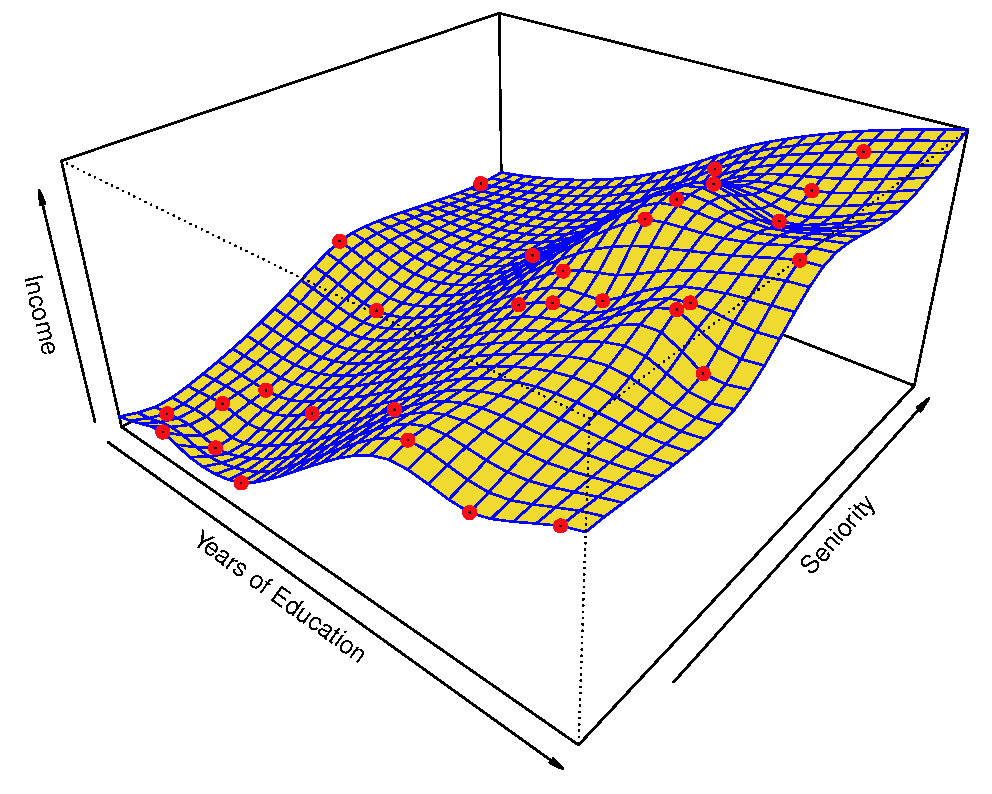
\includegraphics[width = \textwidth]{2-6.pdf}
    \end{column}
  \end{columns}
\end{frame}


\begin{frame}{\normalsize Prediction Accuracy vs Model
Interpretability}

\placefig{0.2}{1}{width=12.2cm}{2-7.pdf}

%\centerline{\includegraphics[width=.9\textwidth]{{{../figures/book_figures/Chapter2/2.7}.pdf}}}
\end{frame}


\end{document}


%\input{temp.tex}